\begin{figure*}
  \centering
  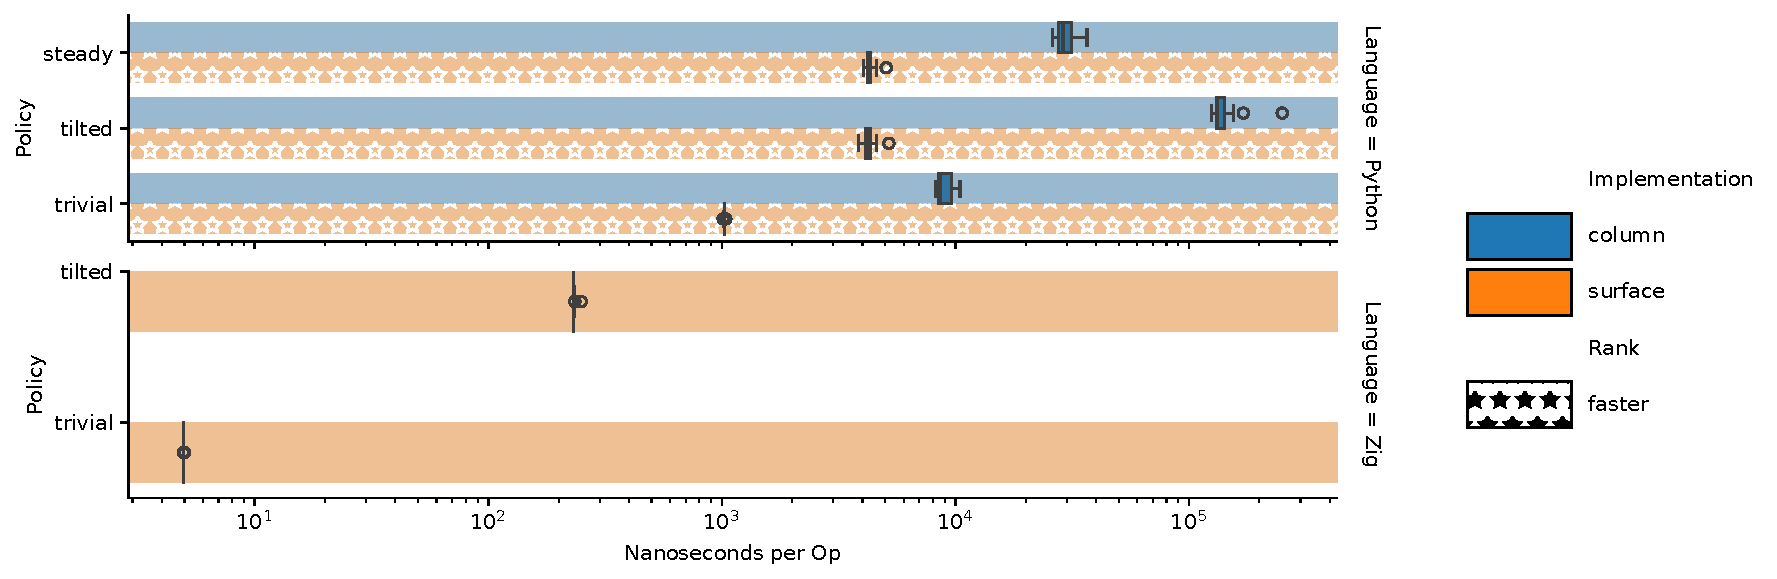
\includegraphics[width=0.85\textwidth,trim={0 0 0 0.4in
  }, clip]{binder-wafer-scale/binder/teeplots/all=false+hue=implementation+orient=h+row=language+score=nanoseconds-per-op+viz=peckplot+x=nanoseconds-per-op+y=policy+y-group=outer+ext=}

\vspace{-2.5ex}

  \caption{%
    \textbf{Hereditary stratigraphy algorithm benchmarks.}
    \footnotesize
    Comparison of per-generation operation time for column- and surface-based steady and tilted retention policies, lower is better.
    Top and bottom panels show Python and Zig implementations, respectively.
    Trivial is a simple hardcoded retention decision, provided as a baseline control.
    Background hatching indicates significant outcomes (Mann-Whitney U test; $n=20$).
  }
  \label{fig:benchmarking}
  \vspace{-0.2in}
\end{figure*}
